% This file is isea.tex. It contains the formatting instructions for and acts as a template for submissions to ISEA 2025. It is based on the ICCC formats and instructions. It uses the files isea.sty, isea.bst and isea.bib, the first two of which also borrow from AAAI IJCAI formats and instructions.
% Modified from ICCC.tex by B. Bogart

\documentclass[letterpaper]{article}
\usepackage{isea}
\usepackage[pdftex]{graphicx}
\usepackage{times}
\usepackage{helvet}
\usepackage{courier}
\usepackage[numbers]{natbib}
\pdfinfo{
/Title (Art as Technology)
% /Author (Kynan Stewart Hughes)}
/Author (Anonymous)}
% The file isea.sty is the style file for ISEA 2025 proceedings.
%
\title{Art as Technology v0.2.2}
\author{Author: Anonymous\\
School: Anonymous\\
Institution: Anonymous\\
Location: Anonymous\\
Email: Anonymous\\
% \author{Kynan Stewart Hughes\\
% Creativity and Cognition Studios\\
% University of Technology Sydney\\
% Sydney, Australia\\
% kynan.s.hughes@student.uts.edu.au\\
\newline
\newline
}
\setcounter{secnumdepth}{0}

\begin{document} 
% Setting the default tolerance level
% \tolerance=200
% Setting a high tolerance level
% \tolerance=10000
% Some more drastic measures for hbox issues
% \emergencystretch=4em
% \raggedright
\maketitle
\begin{abstract}

    This paper examines the concept of art as a technology, applying complexity science and Process Philosophy to explore how art objects function as complex adaptive systems of meaning. By positioning art as a technology, the paper challenges the traditional distinction between artistic and technical practices. The analysis draws on complexity thinking to argue that art objects reorder information and generate indeterminate yet meaningful networks. This perspective encourages artists working with emerging technologies to engage with art as a craft of conveying information and context about technology, transforming our understanding of both artmaking and technology.

\end{abstract}

\keywords{Keywords}

Art, technology, complexity, aesthetics, affect, information, craft, systems, emergence, meaning, constraints, coarse-graining

\section{Introduction}

    Over the last 80 years, the concept of complexity has emerged as a kind of meta-theory based on the idea that mostly everything can be thought of as a complex system made up of complex systems situated within and across the fuzzy, overlapping boundaries of other complex systems. Everywhere we look we see things interacting in ways that would have been impossible to predict, and when we look more closely we see that the things themselves are nothing more than the emergent approximations of interactions between things that are themselves fleetingly stable regularities in a ceaselessly changing, sometimes ordered, sometimes chaotic flux. Nothing exists independently. Everything is overlapping and connected and only momentarily and contingently stable. All is process.
    
    Complexity thinking is the awareness of “the epistemological consequences of assuming the ubiquity of complexity” \citep{CilliersRichardsonCmplxtyScnc2001}. In other words, it changes what we think it is possible to know, while at the same it radically changes the possibilities for knowing. It is a kind of not knowing that is closer to understanding.
    
    In science, rapid developments in theories of complexity over the last several decades, including Chaos Theory, Dynamical Systems Theory, and Complex Adaptive Systems Theory, constitute nothing less than a paradigm shift away from simplistic, deterministic, clockwork models of the world and towards a view that embraces unpredictability, interdependence, and emergence \citep{StengersOrdrOtOfChs1984}. The ancient Western tradition of process philosophy \citep{SeibtStnfrdEncyclpdPrcssPhlsphy1974} has been invigorated by this change, absorbing knowledge from science and mathematics, and contextualising it within a sophisticated materialist ontology that connects all aspects of material and human social activity and thought, including (of course) art and technology.
    
    This paper draws on both scientific theories of complexity and theories of art and of technology that are influenced by process philosophy. It is an experiment conducted at the boundary between art and technology which has implications, especially, for artists who work with emerging technologies.
    
    It starts from the idea that art is a technology.

    We have an edge against the idea of thinking about art as a technology. It just feels weird\footnote{
        The idea of art as a specific kind of technology only rarely appears in the literature around art, even in the tradition of materialist process philosophy. When Giles Deleuze and Felix Guattari used the term “machine”, even in the context of “aesthetic machines” \citep[p.42]{GuattariChsmss1995} it was in a sense that covered all kinds of “machinic assemblage” \citep[p.41]{GuattariChsmss1995}, not technical machines specifically. When Stephen Zepke, quoting Deleuze, announced that “art as abstract machine will require an artist adequate to the task: a mechanic. For each machine its mechanic: ‘The painting machine of an artist-mechanic’" \citep[p.1]{ZepkeArtAsAbstrctMchn2005}, he was being clearly metaphorical. Simon O'Sullivan was perhaps going beyond metaphor and beyond the machine of Deleuze and Guattari when he called art an “aesthetic event-based technology” \citep[p.202]{ZepkeOSullivanDlzCntmprryArt2010}, but he did not elaborate. Anne Sauvagnargues, in her book \emph{Artmachines}, drawing parallels between Deleuze’s ideas on art and Gilbert Simondon’s concept of the technical object, has explicitly suggested that art operates as a kind of technology — one that modulates forces and generates meaning. “Art as technics”, she wrote, ”concerns the way in which materials (matières) are captured and assembled into matter (matière) of expression.” \citep[pp.74-75]{SauvagnarguesArtmchns2016}. However, the implication of thinking about art as a technology are not explored deeply in \emph{Artmachines}. The book is more concerned with idea of art as a kind of “machine” in the way Deleuze and Guattari frequently used the term.
    }, and perhaps a little bit risky. It is as if art needs to be protected from such a move. Perhaps we fear that thinking of art as a technology will destroy the special qualities of art and reduce its value as a practice. This paper explores the potential for another outcome in which the idea of art as a technology leaves art as we know it intact but expanded, and opens new possibilities for how we make sense of \emph{technology}. Helping us to see our technologies differently is one job that artists who work with emerging technologies can do. The slogan “Art as Technology” is proposed as a kind of heuristic for creative technologists of all kinds, opening a space of possibility for thinking and making differently with art and with technology.

\section{A definition that can be applied to all technical objects} 

    According to Brian Arthur a technological object is always “a phenomenon captured and put to use” \citep[p.53]{theNatureOfTechnology2009} or, put another way, “a programming of phenomena for a purpose.” \citep[p.53]{theNatureOfTechnology2009}. This distillation holds for the full range of diverse technologies, contemporary and historical.

    Phenomena don't have to be physical phenomena like fire or electricity. They may be “behavioural or organisational ‘effects’” \citep[p.55]{theNatureOfTechnology2009} or “truism[s] of nature” \citep[p.45]{theNatureOfTechnology2009}.
    
    We might update Arthur's definition of technology by applying biologist and complexity scientist Jessica Flack's concept of \emph{course graining} in place of the more vague idea of “phenomena”. 

    According to Flack, \emph{coarse-graining} occurs when a subsystem with apparently emergent properties is treated as a single entity by components of the system for predictive purposes. Course graining is a way for components of complex systems (like people) to treat other elements the system that works but ignores many of the details. It is a “lossy but true” \citep[p.4]{FlackCrsGrnng2017} strategy.
    
    Flack has used the idea of temperature \footnote{

        Flack has remarked that this example comes from \emph{Inventing Temperature} by Hasok Chang \citep{ChangInvntngTmprtr2004}

    } to explain the kind of coarse-graining scientists do as a normal part of scientific practice.

    \begin{quote}
        Temperature is the average speed of particles in a system. Temperature is a coarse-grained representation of all of the particles' behaviour — the particles in aggregate. When you know the temperature you can use that to predict the system's future state better than you could if you actually measured the speed of an individual particle. \citep[p.4]{FlackCrsGrnng2017}
    \end{quote}

    Coarse graining is "how adaptive systems identify regularities in evolutionary or learning time and use these perceived regularities to guide behaviour."\citep[p.2]{FlackCrsGrnngAsDwnwrdCstn2021}. It is happening all the time in every system, whether it is physical or social, from coral reef formation \citep[p.61]{FlackEtAlTmsclsSymmtryUncrtnty2013} to the way monkeys establish social hierarchy \citep{FlackCntxtMdltsSgnlMnng2007}.

    All apparent phenomena are the result of coarse graining. Course-graining describes how emergence happens — or at least something about its necessary conditions. A property like temperature emerges, through processes that include course-graining, from interactions between physical substances, people measuring, systems and devices of measurement, and the environment. A distribution of relative status ‘scores’ in a monkey group emerges, through processes that include coarse-graining, from a system of signalling interactions between individual monkeys and the perception of those signals by the group \citep{FlackCntxtMdltsSgnlMnng2007}.
    
    We might say then, that a technological object is a programming of \emph{perceived regularity} for a purpose.

    For example, money is a technology because it depends on a perceived regularity of human behaviour, which is the trust people put in tokens of value.

    \begin{quote}
        The monetary system makes use of the “phenomenon” that we trust a medium has value as long as we believe that others trust it has value and we believe this trust will continue in the future. \citep[p.55]{theNatureOfTechnology2009}
    \end{quote}

    We have established a general definition of technology that can be applied to all technical objects, and we can now perhaps start to experimentally apply this definition to art objects. However, before we do that, we need to establish a general idea of what art is — or, rather, we need to be clear about which of the many overlapping ideas about art we mean when we say “art”.

\section{The Aesthetic Regime}

    Jacques Rancière has called the currently dominant idea of art the \emph{aesthetic regime}. It is not a single coherent paradigm, but a “plurality” of “frequently different, and sometimes contradictory, ways of thinking” \citep[p.8]{RanciereMdrnTms2022} about art organised around the idea of aesthetic experience. This is a radical repositioning of Aesthetics as art itself, rather than as a theory about art.
    
    The aesthetic regime emerged at the end of the eighteenth century with Emanuel Kant's \emph{Critique of Judgement} and some other key texts that followed it. Kant's radical break was to propose that the essence of an art object lies in its capacity to be experienced without concept. With the clarity of hindsight, we can see as Rancière did, that it is the separation of sense-as-in-sensation and sense-as-in-making-sense which created our current situation in which the effectiveness of an artwork, the very thing that makes it art, is “a paradoxical kind of efficacy that is produced by the very rupturing of any determinate link between cause and effect.” \citep[p.51]{RancierThEmncptdSpcttr2009} ”It is precisely this \emph{indeterminacy}\footnote{
        My emphasis.
    }”, he said, “that Kant conceptualized when he defined the beautiful as ‘what is represented as an object of universal delight apart from any concept’. \citep[p.52]{RancierThEmncptdSpcttr2009}

    The purpose of an artwork (we might call it \emph{meaning} since they amount to the same thing for artwork) is always organised around aesthetic experience. This constraint is the origin of art's autonomy within Modernity and the source of all possibility with respect to how art and art objects can interact with other aspects of Modernity, including all potential for generating meaning or taking political action, for example. All distinctions and differences within the idea of art operate within the aesthetic regime. Ideas about Modern and Post-Modern art, for example, are different, perhaps contradictory strategies for trying to do something worthwhile within the aesthetic regime \citep[p213]{ZepkeSblmArt2017}. Art which is anti-aesthetic, for example, is still operating within the aesthetic regime in a way that is self-consciously critical of it (in fact, because of that). Conceptual art is art that invites us to consider the aesthetic potential of ideas\footnote{
        Reference needed?
    }.

    One of the key features of the aesthetic regime is that it enables objects created under other regimes — for purposes other than aesthetic appreciation — to be experienced as art. As Marcel Duchamp proved in 1917 when he entered a urinal into an art exhibition, and as has been proven many times since by practitioners of the style known as Contemporary Art for whom the readymade is a key strategy, there is nothing in the world that cannot be made into a work of art even by the simple act of declaring it to be one. A kind of transfiguration, or dislocation, occurs when an object is brought into the aesthetic regime. The object is no longer understood in terms of its original function or purpose, but as an object of contemplation within the aesthetic regime. “The aesthetic regime”, as Rancière put it, “asserts the absolute singularity of art and, at the same time, destroys any pragmatic criterion for isolating this singularity. It simultaneously establishes the autonomy of art and the identity of its forms with the forms that life uses to shape itself.” Literally anything can be art. It is not simply that objects \emph{can} be transfigured into art objects, but that the aesthetic regime \emph{is} a system of codes that dislocates objects from their original functions and meanings. This “dissensual operation” of creating an artwork, for example by working materials into forms, by organising sounds in certain ways, by setting the state of pixels on a screen, by isolating and performing specific movements with our body, or by appropriating a ready-made object, “transforms a given form or body into a new one.” \citep[p.54]{RancierThEmncptdSpcttr2009}.

    Having established that the term “art objects” applies to materials or even pre-existing objects encoded into the aesthetic regime, we can begin to tentatively apply our definition of technology as \emph{the programming of perceived regularity for a purpose}. A question immediately arises: what perceived regularity do art objects capture?

\section{From Beauty to Affect}

    The concept of \emph{affect}, which comes from Deleuze and Guattari via Brian Massumi, is a way of thinking about how things affect other things in the complex systems of interconnections material reality, including the way that our bodies and minds are affected by the world around us. Affect is a kind of intensive, interactive event. Affect happens between us and the world and is always also going on all around us. It is in no way limited to being human. It is human and inhuman, organic and inorganic. It is the way that we and things are moved by the world and each other. It is a pre-cognitive, pre-linguistic, pre-conscious event during which the world emerges into existence. Perceived regularities happen when affect happens.
    
    In a reality that consists entirely of unfolding processes, objects are processes that stay still long enough to be noticed. Objects come into existence for us through processes of coarse-graining, which are both material and social. Objects are \emph{slow variables} — that is, they are “...macroscopic states that...change slowly with respect to the underlying dynamics generating the state...” \citep[p.61]{FlackEtAlTmsclsSymmtryUncrtnty2013}. Once called into existence, objects seem to embody the affective properties and capacities — the \emph{estimated regularities} \citep[p.9]{FlackCrsGrnng2017} — that caused them to appear.

    For Kant, the range of aesthetic experience as it pertains to art objects was limited to the experience of beauty\footnote{
        He also, at the last moment, included ‘the sublime’ \citep[p.15]{ZepkeSblmArt2017} as that which is experienced as a kind of rapid toggling back and forth between fear and pleasure \citep[p.88]{KantCrtqOfJdgmnt} because of its infinitude. There is some evidence in \emph{Critique of Judgement} to support the idea that this kind of experience might be produced, however indirectly, by a constructed object like, say, the pyramids \citep[p.82]{KantCrtqOfJdgmnt}, although it is not entirely clear whether Kant actually thought this is possible or whether he was allowing that experiences of the sublime might pertain to artworks. In any case, including the sublime in the short list of two kinds of affect that art objects might engender simply reinforces the point that it is a very short list.

    }. These days, an exclusive focus on beauty when it comes to aesthetic experience and art, is starting to seem like a strangely unnecessary limitation to put on aesthetic experience and on art \citep[pp.121-122]{HighmoreBttrAftrTst2010}. Contemporary scholars, coming at aesthetics from the perspective of affect, note that the field of Aesthetics had been developing for 40 years or so before \emph{Critique of Judgement} was written and that its remit was always more broad than experiences of beautiful art\footnote{
        The inception of aesthetics as a field is attributed to European philosopher Christian Wolff and his disciples, including Moses Mendelssohn and, especially, Alexander Baumgarten. Baumgarten thought that the Cartesian philosophical emphasis on logic and conceptual thought had neglected the epistemological role of sensorial experience. For him, aesthetic cognition mediated between reason and sense; the aesthetic was a kind of (inferior, feminine) analogue of reason, operating at the level of material life \citep[pp.327-338]{EagletonFrPrtclrs1990}. 
    }. The entangled dualism that aesthetic experience should be mainly limited to experiences of art and that these experiences should be limited to beauty now seems naive\footnote{
        Ben Highmore, in the context of arguing for a more expanded view of aesthetic experience as synonymous with affect, has pointed out the historical logic connecting beauty and art as a morally uplifting activity \citep[p.121-122]{HighmoreBttrAftrTst2010}. Baumgarten thought that, within the dense amorphous flow of our sensuous experience constantly in flux, certain objects stand out in a kind of ideality akin to rational perfection, which is beauty \citep[p.328]{EagletonFrPrtclrs1990}. It makes sense, Highmore suggests, that beauty should become the approved affective experience for art objects, because art was a kind of moral training for the soul, and beauty was the most morally uplifting affect.
    } The recent move to equate aesthetic experience with affect is a shift away from the idea that some normative experiences — like beauty, for for example — are better than others, and that the artwork is a moral lesson, and towards the messy reality of material processes. It contextualises aesthetic experience in a complex ecology of affect. As Ben Highmore put it, referencing Felix Guattari, art is now about “complex affective and intensive exchanges, situated in the broader ecology of the world.” \citep[p.155]{HighmoreBttrAftrTst2010}

    Humans, because of our cognitive and social peculiarities\footnote{
        Reference needed - \emph{The Symbolic Species} by Terrence Deacon
    }, are particularly good, perhaps a little too good, at attributing affective regularity to objects, and this is the perceived regularity that art objects capture. We see faces in clouds, spirits in trees, and stories in rocks. Art is a system of coding that both constrains and amplifies this capacity. Codes of the aesthetic regime govern the production, distribution, and reception of objects that have been called art. Through this process of amplification, art objects become charged with affect. They are slow variables packed with potential affects, like batteries holding a charge.

    The affective charge of an art object can consist of any complex combination of qualities, including qualities that are strong, weak, sensorial, semantic, abstract and indeterminate. It can be a sense of the beautiful, or it can involve concepts and feelings that are much more difficult to pin down. Art can be uncanny, ridiculous, tragic, comic, horrific, erotic, sacred, profane, boring, transcendent, immanent, infinite, eternal, historical, present, immediate, distant, and so on without limit. It can, like a Patricia Piccinini sculpture, strobe between incompatible affective states, such as the cute and the grotesque. Like Duchamp's readymades, it can call attention to the affective charge of art itself.

    Art, the aesthetic regime, is system of codes that dislocates objects and materials from their original functions, and meanings, and programs them with new affective potential. It is essentially a hack on our capacity for affect. It is a kind of technology that encodes — or \emph{programs} — our capacity to attribute affective potential to objects. The terms “artworks” and “art objects” apply to materials, even pre-existing objects, programmed by the art with fresh affective potential.
    
\section{The purpose of art}

    Having experimentally placed technology and art on a plane of consistency via the concept of \emph{the programming of perceived regularity}, the question of \emph{purpose} remains. If we are to continue the experiment of thinking of art as a technology, we must consider the purpose of art objects and whether the nature of the relationship between the programming of perceived regularity and purpose in art objects is in any way different enough from the nature of purpose in technical objects to separate artmaking as a set of practices from technology as a different set of practices.
    
    The purpose of a technological object is its intended use, which must be something one step away from the effect of the perceived regularity is programs. For example, we can't say that the purpose of a match is to spark into flame because its capacity to spark into flame is the perceived regularity that is captured by match technology. The purpose of match technology is the use to which that capacity is put, which is to start another fire. 
    
    % A male bowerbird crafts a bower which generates affect for a female bowerbird, so the purpose of a bower is (speaking evolutionarily) to enable sexual reproduction\footnote{
    %     Elizabeth Grosz
    % }. If, as Deleuze and Guattari suggested, human artmaking has its evolutionary origins in theses kinds of activities, then surely we are unique among animals with respect to the diversity of affective objects we craft. 

    Arthur Danto said that artworks are “embodied meaning”\footnote{
        Reference needed.
    }, and meaning is a useful way to think about the general purpose of art objects as long as we are clear about the meaning of “meaning”.
    
    In saying that art objects embody meaning we run the risk of conflating or confusing two different uses of the word “meaning”. Manuel DeLanda has pointed out that the word meaning in the expressions “this word has a meaning” and “this life has a meaning” are two entirely different words, and that “using them as if they were the same word can lead to erroneous conclusions. In particular, it may lead to the mistake of thinking that everything around us, everything that makes us feel relevant and capable of making a difference, is a linguistic matter, and therefore that our activities are nothing but an enacted text.” \citep[pp.40-41]{DeLandaCsltyAndMnng2018}
    
    It is better to be more specific and say that art objects embody \emph{context} because context is the origin of the kind of meaning we mean when we talk about art. Massumi has said, “meaning is [...] a network of enveloped material processes” and, quoting Deleuze and Guattari, “‘A thing has as many meanings as there are forces capable of seizing it.’” \citep[p.10]{MassumiAUsrsGdTCptlsmAndSchzphrn1992}.

    Context, in terms of complexity thinking, is an important concept because complex systems are always complexly situated in overlapping and nested relationships with other systems. Context is roughly synonymous, in scientific terms, with the control space of a system\footnote{
        Reference needed — DeLanda.
    }, which is integral to the probability space of the system's possible states — or, the “state space” of the system. And art objects are, like most things, complex systems. One way to think about the way art objects fulfil their purpose of embodying meaning is to think about how they function as complex systems in relation to their context.
    
    Jason Hoelscher has pointed out that art objects are epiphenomenal, like rainbows \citep[p.17]{HoelscherArtAsInfrmtn2021}. It is always possible to see how they are the result of some other phenomena. The materials from which they are made are always visible, and yet the artwork exists somehow separately from these materials. An art object is made, in a way, out of its own \emph{artness}.
    
    \begin{quote}
        [...] a work of art is a complex adaptive epiphenomenon of its own manner of phenomenalization: the penumbra of indeterminacy around an artwork is what defines it as an artwork, and is not only the effect of its mode of instantiation but also its cause. In other words, art is a self-ramifying process, an unfinalizable feedback loop \citep[p.2]{HoelscherThPtcsOfPhsSpc2014}
    \end{quote}

    In Hoelscher's formulation, art objects are indeterminate because they are, as Kant suggested, “purposive without a purpose” \citep[p.57]{KantCrtqOfJdgmnt}.

    \begin{quote}
        The claim here is not that art lacks purpose, but that art's purpose is contextually complex and indeterminate, and so remains open to transformation and differentiation by lacking external, objectively shared criteria by which to resolutely judge or interpret the work. Lacking this anchor of specificity, art's purpose remains expansive, many layered, and multidimensional.\citep[p.25]{HoelscherThPtcsOfPhsSpc2014}
    \end{quote}

    Objects instantiated as artworks remain indeterminate in that their meanings are not fixed because it is always susceptible to shifting context. The shifting meanings attributed to art objects over time and in different contexts are “a series of attractor basins in possibility space” \citep[p.4]{HoelscherThPtcsOfPhsSpc2014}
    
    \begin{quote}
        Being unfinalizable and open, and manifest via the tautology of purposiveness without purpose, an artwork draws the viewer toward possible interpretations while nonetheless preventing a fixed, final understanding. It is this epistemological opening around which the artwork-as-attractor basin accretes, around which a swarm of interpretations are possible but never definitively attained. \citep[p.12]{HoelscherThPtcsOfPhsSpc2014}
    \end{quote}

    It has been suggested that information is for complexity science what energy is for classical physics\footnote{
        “In physics the sort of dominant object or concept or entity we”re interested in is energy. And certainly there are many successful applications of more or less traditional physics — say, the physics of phase transitions — to complex systems. But many of these complex systems if we”re thinking of social networks or a human-designed systems the internet, don”t necessarily have an appropriate notion of energy, so information in many ways stands in for trying to describe how complex a complex system is. Various kinds of information processing and storage can be associated with how a system is organized.  So it”s a key concept.” \citep[0:52]{CrutchfieldIntrdctnToCmplxty2018}
    } \citep{CrutfieldRtAlSgntrsOfInfnty2015}, and it is central to Hoelscher's theory of art. He has blended Claude Shannon's Information Theory with Gilbert Simondon's idea of information arising from meaningless disparity as emergent, meaningful difference. Hoelscher summed up Simondon's concept of information as the “relational operation of difference that intensifies or generates a context”. He has described art objects as sources of information because they are open to interpretation — that is, they are interpreted relative to a context. 
    
    % Hoelscher has reminded us that information was shown by Shannon to be a function of the relative entropy of a system — that is, the total available entropy (all the possible states of a system in a given context) minus the actual entropy (the actual state of the system). He has pointed out that entropy is a form of symmetry, using the example of a white cue ball as an example of an object that is symmetrical with respect to rotation.
    
    % \begin{quote}
    %     [...] Entropy is a form of interchangeability. Interchangeability is another word for an extreme degree of symmetry: the white cue ball can be rotated, rearranged, flipped, and so on without notable difference in appearance, because its surface areas are extremely symmetrical and interchangeable — entropic, in other words. \citep[p.4]{HoelscherThMxmmPtntlEntrpy2017}
    % \end{quote}

    % Since “information for Shannon is a measure of the surprise, or difference from expectation, created when a difference emerges into, or travels through, a context” \citep[p.6]{HoelscherArtAsInfrmtn2021}, with respect to changes in rotation there is no information in this cue ball system. 
    
    % However, where there is a lack of symmetry, there is information. We might imagine a cue ball that suddenly develops a single protruding bump. Now, relative to rotation, the system is not symmetrical. This would be an entirely new system in which information is possible. As Hoelscher points out, “information for Simondon is a relational operation of difference that intensifies or generates a context” \citep[p.6]{HoelscherArtAsInfrmtn2021}. 

    The resolution of meaningless disparity into meaningful difference is not a process that is peculiar to art. It is the process by which all things come into existence. It is everywhere and always a wildly creative event that results in an exponentially more vast field of potential for meaningful action — a huge increase in capacity to affect and be affected. Hoelscher has invited us to consider, for example, the evolution of eyes from, perhaps, light-sensitive areas on an organism's surface, that eventually become sensitive enough to allow the creature to perceive (on some unconscious level) a consistent (regular) difference in the input signal from different eyes. Suddenly, in the macro-scale equivalent of a quantum shift, a three dimensional universe comes into existence.

    \begin{quote}
        This slight distance between one eye and the other causes two distinct visual streams, which resolve into the rich depth perception of binocular vision. Here, the reconciliation of a simple disparity yields a result far more complex than one might expect, given the small scale of the initial problem. \citep[p.5]{HoelscherArtAsInfrmtn2021}
    \end{quote}

    Since an art object never settles into one particular, fixed state of communicated meaning, it is an open-ended, endlessly generative source of information \citep[p.7]{HoelscherThPtcsOfPhsSpc2014}. As Hoelscher has explained it, art is tapping into the generative power of the universe itself, which is always creating information.

    These epiphenomenal art objects grab our attention by their virtue of their complex, contingent mode of existence.

    \begin{quote}
        An epiphenomenon [...] foregrounds its existence not as a resolute or finished thing but as the ongoing operational contingency of itself, as itself. Whether in the guise of a rainbow or an artwork, the strangeness of this perceived contingency — of a sustained process of focused incompletion taking place right before our eyes — compels us to stop, look, and linger.
    \end{quote}

    Once they have our attention, these “differentially complex” \citep[p.74]{HoelscherArtAsInfrmtn2021} objects make information available that is otherwise hidden in plain sight as apparently disordered, entropic chaos.
    
    Far from being a non-ordered type of entropy, the disorder of the world is “a highly charged and catalytic mode of entropy akin to information entropy — not inert, but saturated to bursting with potentials that are oriented toward actualization.” \citep[p.72]{HoelscherArtAsInfrmtn2021}. Disorder, he says quoting Henri Bergson, “is simply an order we are not looking for.” \citep[p.73]{HoelscherArtAsInfrmtn2021}. Within this milieu, potential orderings “bustle and crackle”, awaiting “catalytic discharge upon their convergent processing through the differential gap.” \citep[p.73]{HoelscherArtAsInfrmtn2021}, which “sheds information that shows up as a difference that makes a difference.” \citep[p.75]{HoelscherArtAsInfrmtn2021}. Helpfully, Hoelscher provided a number of examples.

    One example is the hyper minimalist sculptures of Robert Morris, which are simple grey cube-like forms placed directly on the floor of a gallery.

    \begin{quote}
        By giving the viewer so little to look at, Morris [...] directs the flow of attention away from the object itself and toward the object's relations with the gallery space, with the changes of light and shadow over time, and with the viewer's field of experience as an experience in and of itself. Accordingly, with the severe reduction of the work's surface qualities, internal differentiations, particularity, and variability, the artwork and its local situation fold into one another — a direct ingression of the differential information object into the space of lived experience. \citep[p.78]{HoelscherArtAsInfrmtn2021}
    \end{quote}

    Another example is a Duchamp readymade. Describing \emph{In Advance of the Broken Arm} (a snow shovel) Hoelscher said:

    \begin{quote}
        [...] the readymade's enfolding of object and idea activates (and is activated by) a wide-ranging network of differential tensions between the object and its context, and between cultural, historical, and artistic expectations regarding shovels, artworks, and the application of artistic skill [...]
    \end{quote}

    This is nothing we haven't heard before with respect to a Duchamp readymade. What is interesting is that functioning of both the Morris sculpture and the readymade, their embodying of meaning, is described in terms of existing information reordering around them as art objects. The information in each case is very different. The Morris sculpture reorders information around the object's relation to the gallery space, light and shadow, and the viewer's experience. The Duchamp readymade reorders information around the object's relation to the history of art, the history of shovels, and the history of Duchamp's own work. The information that is reordering is different, but the process is the same.

    Alicia Juarrero's concept of \emph{enabling constraints} is especially useful as a way to think about meaning as context because it gives artists something to grab onto and work with.
    
    Juarrero has identified two types of constraints that define the probability space of complex systems: context-free constraints and context-sensitive constraints. In terms of information, both types of constraints are necessary for reducing randomness in order to separate information from noise but, she says, only context-sensitive constraints enable signals that convey meaning. While both types of constraints function by limiting possibilities, context-sensitive constraints also create possibility by connecting a simple message/information system that is initially defined by context-free constraints with the complex systems in which it is embedded.
    
    Unlike context-free constraints which simply limit the potential states a system can be in, context-sensitive constraints also create new dimensions of possibility by connecting the system with the state-spaces of other systems. Context-sensitive constraints are another way to explain emergence. \citep[p.240]{JuarreroCsltyAsCnstrnt1998}.

    Juarrero has illustrated the way enabling constraints operate to create context by describing a lighthouse\footnote{

        Juarrero attributes this analogy to Bob Artigiani.

    } as an information channel.
    
    A lighthouse it is physically constrained to having only two possible states — it can only blink on and off. Without any other context — say, when it is seen by a Martian on mars — the sequence of signals from a lighthouse amounts to transmitting “Message”, “Message”, “Message”. The message contains information but it has no meaning. The meaning comes from the constraints that connect the flashing light with a broader network of things and events.

    \begin{quote}
        It is because of his awareness of a network of relationships that the sailor, unlike the Martian, can understand that the flashes of light he sees mean "Land!". The sailor sees the flash of light as a node in a complex network of relationships [...] Indeed, the sailor is a sailor (and not just a man adrift on a boat) only because he himself is embedded in a network of [contextual] relationships (such as navigation, tacking into the wind, etc). [...] Signals subject to [contextual] constraints refer to the contextual web (temporal and spatial) in which that particular signal or event is embedded. The information such signals or processes carry is of the organization of the network; the actual information content is about the overall web, not just of its components.\footnote{

            I have swapped out Juarrero's technical term “D2 type” for the more friendly “contextual” simile she uses elsewhere in the article.

        } \citep[p.237]{JuarreroCsltyAsCnstrnt1998}
    \end{quote}
    
    If we want to add more meaning to the flashing signal, we need, paradoxically, to impose more constraints on it. For example, Morse code puts strict constraints on a simple on/off signal like a flashing light. Every combination of flashes must amount to one of the 54 symbols (letters, numbers and punctuations) in the code. Because they are code, the signal information is suddenly “of the organization of the network”. Language is enabled by the constraint of Morse code.

    The concept of enabling constraints is another way of describing Flack's coarse-graining. Sometimes the perspectives align, as when Juarrero says that context-sensitive constraints cause parts of a system to interact and produce dynamical structures that are “describable mathematically as collective variables” \citep[p.193]{JuarreroThSlfOrgnstnOfIntntnlActn2004}. Usually though, Juarrero describes this process from the perspective of the constraint rather than the components. Where one might imagine that Flack would say a flashing lighthouse signal is a regularity that for some seafaring groups of people forms part of a slow variable for storing information about safe navigation at sea, Juarrero would say that a flashing lighthouse is connected, through the enabling constraint of Morse code, with the possibility space of language. When enabled by Morse code, the capacity of this lighthouse variable for communicating and storing information is vastly increased.

    The meaning of an art object emerges from the constraints that connect it with a broader network of things and events. The meaning of an art object is the information it carries about the organization of this network. This leads to an interesting and potential heuristic for artists: if we want to add more meaning to an art object, we need to impose more context sensitive constraints on it.

    \begin{figure}[h]
    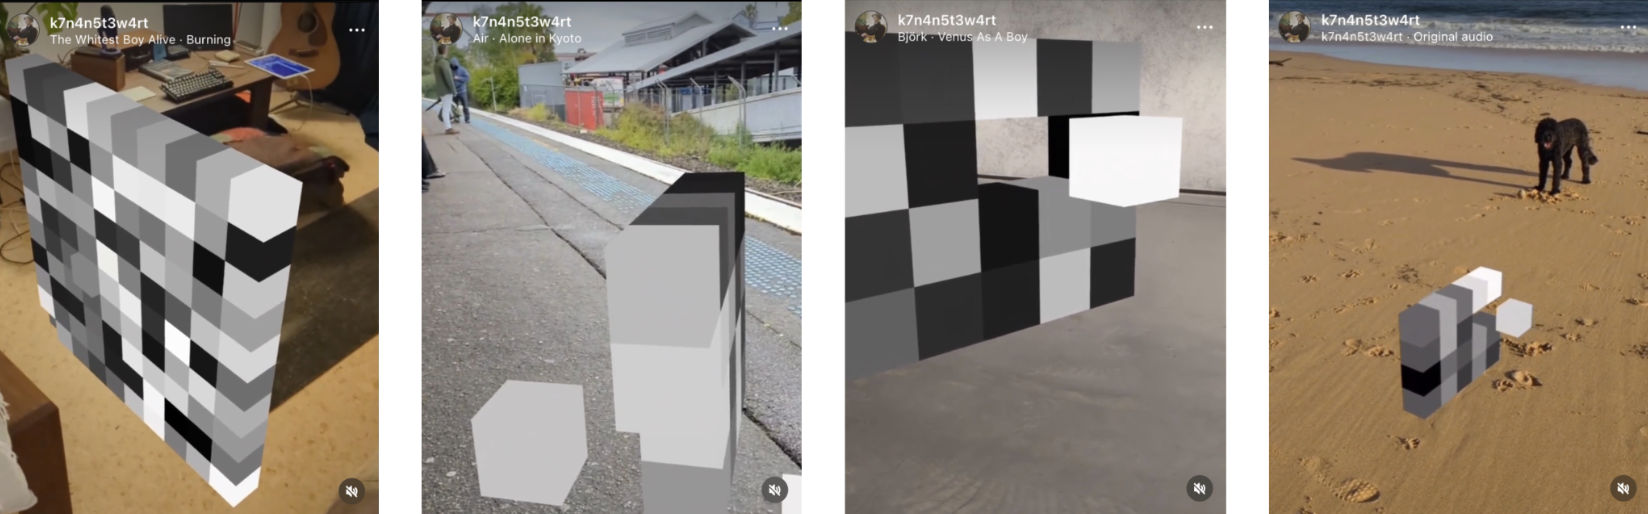
\includegraphics[width=3.31in]{bubble-sort.png}
    \caption{One of the \emph{Algorithm} series called \emph{BubbleSort}. \copyright Respect Copyright.}
    \end{figure}

    For example, a series of augmented reality sculptures I made called \emph{Algorithm} relies on a conceptually simple set of constraints that define the meaning of each piece and the series as a whole. Each piece in the series is single a wall of greyscale blocks. The number of rows and columns in the wall varies, as do the dimensions of the blocks. This is a context-free constraint that produces stylistic consistency but is not meaningful.
    
    Each piece in the series depicts a different sorting algorithm. The blocks sort themselves into a gradient of greyscale shades from lightest at the bottom to darkest at the top, then randomly scatter and the sorting process stars again. The blocks move according to the the algorithm they represent. The algorithm functions as a meaningful constraint, because the qualitative difference between each piece is entirely derived from the way the blocks move. Each algorithm is experienced as having a markedly different quality from the rest. It is also possible to recognise the particular algorithm from watching the way the blocks move. This series explores the resonance these primitive algorithms have in an era where their contemporary descendants organise large portions of our lives. Their simple, hand-made quality references the craft that goes into technical production, even information technology.

    Art, when understood as a complex system of systems, begins to look like a technology that captures the perceived regularity that is our own capacity for affect for the purpose of reordering information and creating meaning. Artists work to tune art objects by imposing constraints on them, enabling them to communicate and store information about the organization of the network of things and events in which they are embedded.

    Purpose is always connected to the affective charge, or meaning, of an art object but it is not limited to it. The affective charge of an art object may be a purpose in itself — it may simply be a beautiful object, or a shocking one. At the same time it may confer status, be an investment, or start a revolution. If art objects have as many meanings (or affects) as there are forces capable of capturing them \citep[p.4]{DeleuzeNtschAndPhlsphy2006}, then we might say the same with respect to their non-affective, or non-art, purpose.

    The affective change of an art object may derive, to some extent, from a non-art purpose, but is never reducible to it. In socially connected art, participatory art, and art that is made to be used (craft), for example, non-art purpose and effective charge are intertwined.

    Affect is one type of excess, or surplus product, of a system. Emergent properties are the result of the interaction of the components of a system, but they are not reducible to the properties of the components. All emergent properties of objects, including aesthetic properties, make objects more than the sum of their parts, as Aristotle said. It is the excess, or remainder, of the system that causes a qualitative shift (a phase-shift) in the system.

    \begin{quote}
        If there were no escape, no excess or remainder, no fade-out to infinity, the universe would be without potential, pure entropy, death. Actually existing, structured things live in and through that which escapes them. Their autonomy is the autonomy of affect. \citep[pp.96-97]{MassumiTheAtnmyOfAffct1995}
    \end{quote}

    Affect is the primary type of emergent property produced in art-objects. Artmaking, Massumi has said, is concerned with “the eventful expression of singularity”. Art ”re-presents” the singular event as “actually expressed (contextual excess or remainder)”, as ”the qualitatively transformative movement it is: as affective” \citep[p.252]{MassumiPrblsFrThVrtl2002}. Should the affective charge of an art object have become effectively reducible to its non-art purpose, it would have ceased to be art.

    \begin{figure}[h]
    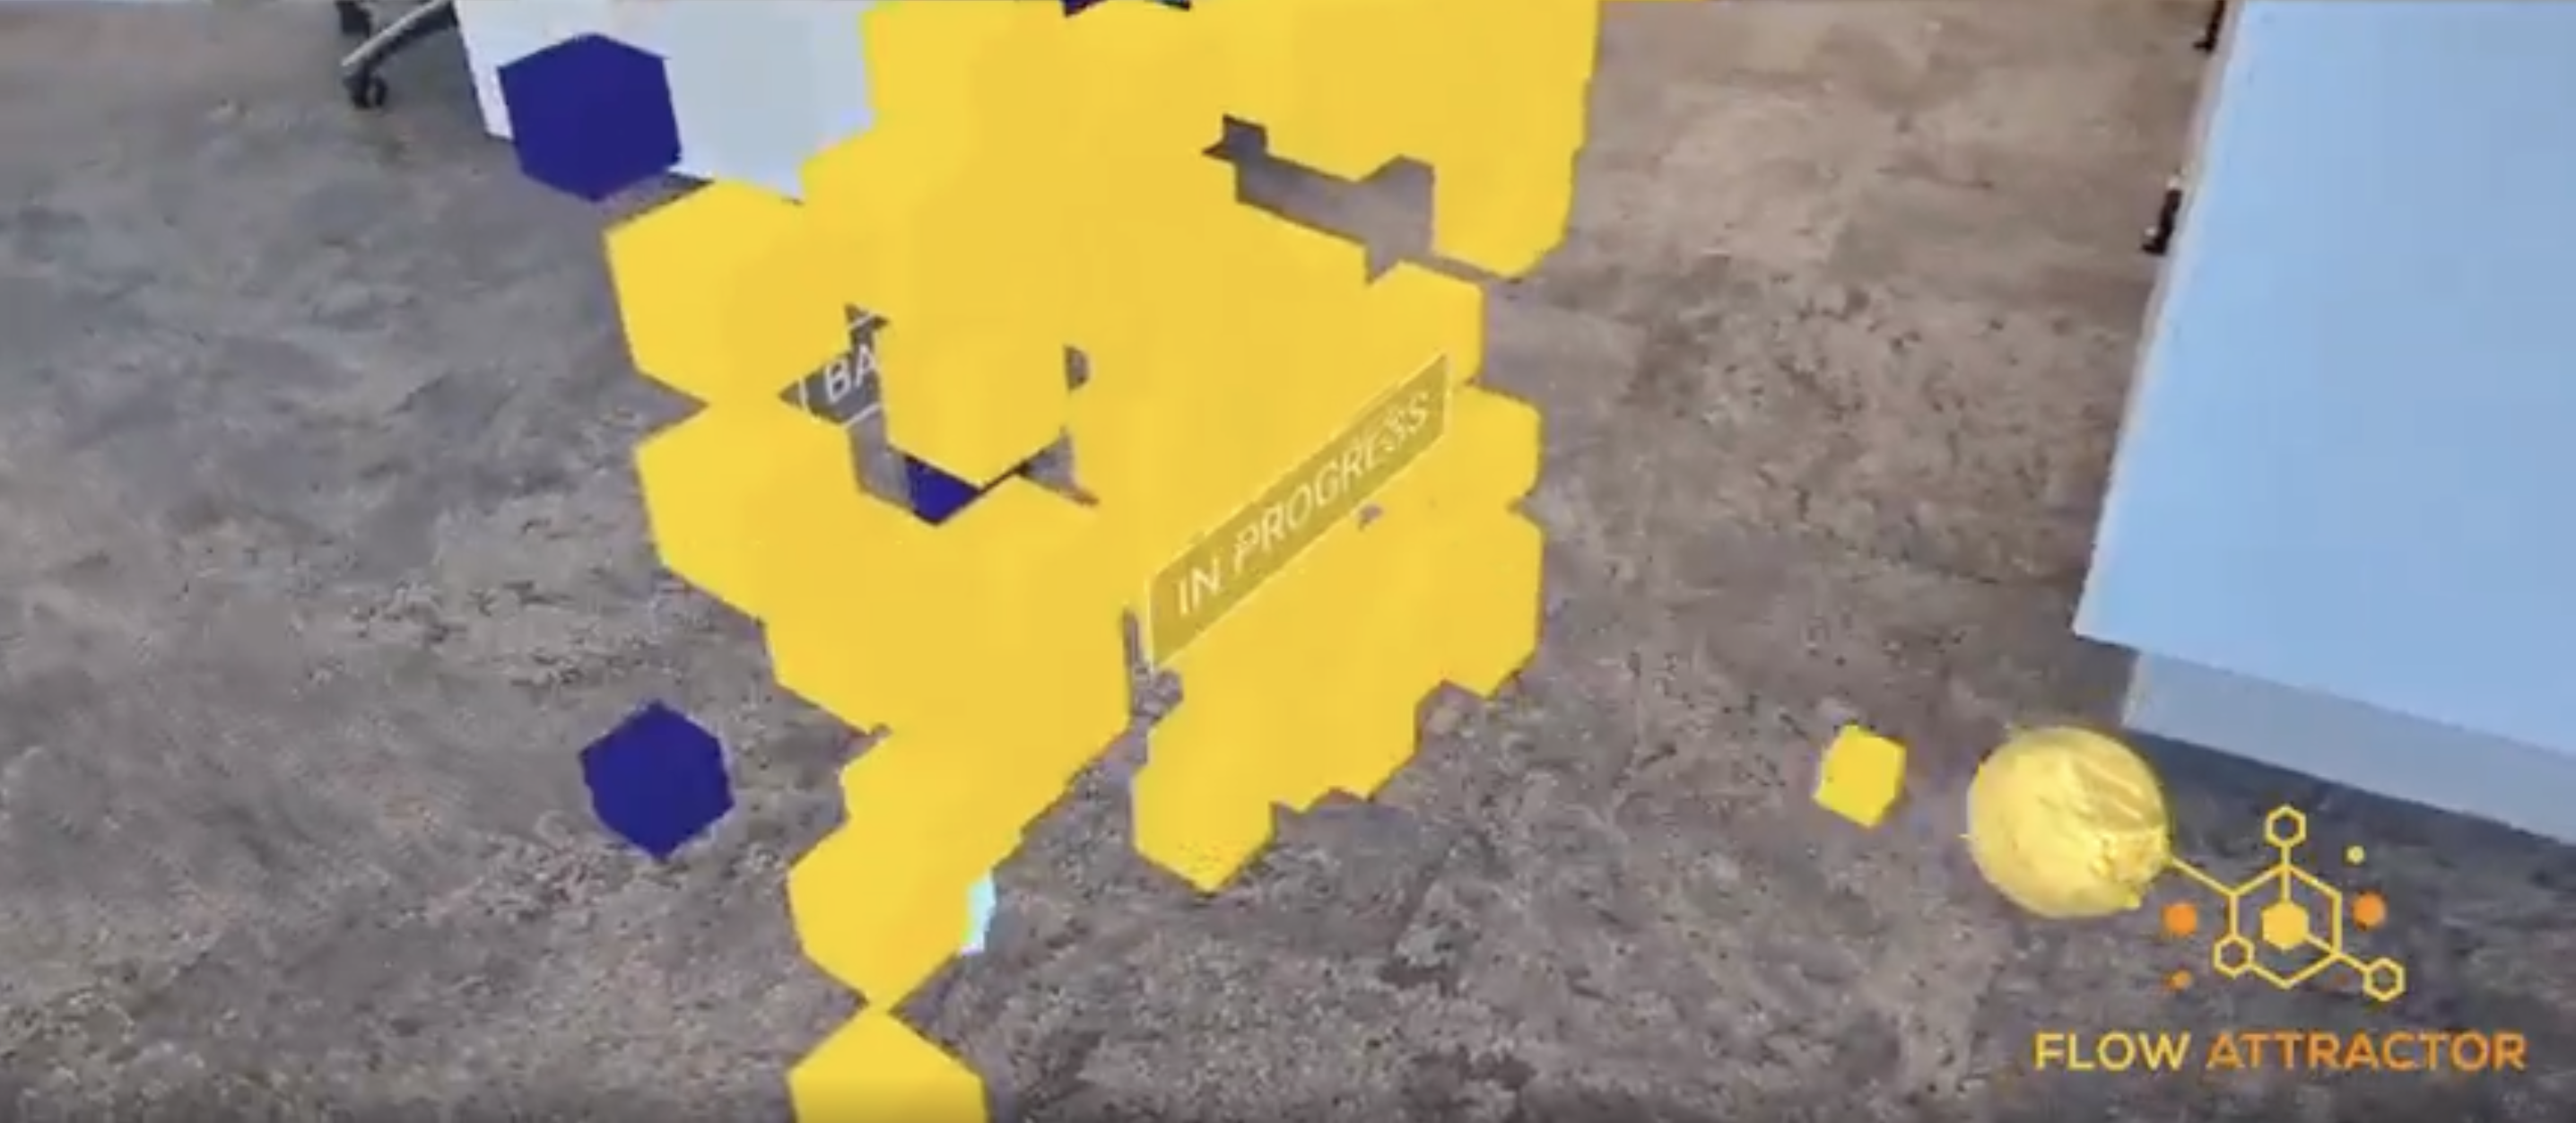
\includegraphics[width=3.31in]{flow-attractor.png}
    \caption{\emph{FlowAttractor} models complex workflows as flying cubes. \copyright Respect Copyright.}
    \end{figure}

    In the piece, \emph{FlowAttractor}, the flow of the blocks represents the otherwise invisible flow of pieces of work - increments of change - through the production system of a large organisation. The piece started as an experiment to find out what would happen if art object was integrated into a business context. The purpose was to catalyse an awareness of the effects of making small changes to the system - managing key constraints - to improve the flow of work through the system. I was trying to generate an experiential shift by using an art-like objects. It worked, but, because the purpose was reducible to a non-art purpose, it was not art.


    \subsection{Indeterminacy of purpose}

    The difference that makes art objects visible as something other than technical objects is the idea that art objects are indeterminate with respect to purpose, while technical objects are not. I want to show that it is possible to think across this difference because it simply isn't true.

    For this to be a true difference, or at least a useful one, technical objects must have determinate (limited and defined) purpose. However, there are plenty of instances in which technical objects are indeterminate with respect to purpose.

    We don't really know how they work. We have a few theories but we will never really know if they are right
    We don't even know how some technologies work - anaesthesia, for example
    
    % They are open to being repurposed - I remember learning that scouts from Disneyland would visit end of year art shows at art schools to find new ideas for animatronic rides. Art is a fantastic R\&D lab for the entertainment industry.
    Technologies are always being repurposed. The internet was originally a military communication system, the microwave was originally a radar system, the purpose of a hammer is to hit nails but it can also be used to open paint tins, and Viagra is an angina treatment.

    % Art objects can have simultaneously overlapping purposes - a water installation at the entrance to the Sydney Opera House, as well as being an artwork, is for cooling the building (I just made that up, there isn't one but there could be). The purpose of a painting is to be a painting but it is also a symbol of wealth and taste, and also a product to be bought and sold. The purpose of a sculpture of a famous person is to be a sculpture but it is also a political symbol of power and authority
    Technologies can have simultaneously overlapping purposes. The internet is for communication but it is also for surveillance, Facebook is for social networking but it is also for advertising, a hammer is for hitting nails and for prising them out, and for being a symbol of the working class.

    Unintended consequences abound - would anyone like to argue that global warming is the intended purpose of the internal combustion engine, or that the purpose of the internet is to make us all miserable, or that the purpose of AirBnB is to make housing unaffordable?
    % Art objects have unintended consequences. When ------- put a huge sculpture called Tilted Arc across a town square in New York, was his intention to make life hell for the people who worked in the surrounding buildings and could no longer use the square? Possibly, but possibly not. Was Christos intention for his umbrella installation in Japan that an umbrella, made airborn by the wind, should impale someone and kill them? Was --------- proposed piece for the Museum of Old and New Art in Hobart Australia, which solicited donations of blood from indigenous Tasmanian people, the descendants of survivors of a genocidal invasion, intended to re-traumatise, outrage and insult them? Apparently, almost unbelievably, it was not. Unintended consequences abound.

    And so we see clearly that purpose for technical objects is contextually complex and indeterminate, and so remains open to transformation and differentiation. Technical objects' purpose remains expansive, many layered, and multidimensional. In this respect, it is the same as art.

    Whichever way we look at the fold of difference between art and technology, it dissolves before our eyes.
    
    Flack has pointed out that course graining is frequently wrong. At best, it is lossy but true. At worst, and frequently, it is just lossy. People are hard-wired to look for pattern, and it has apparently been evolutionarily advantageous to see patterns even to the extent that we see patterns where there are none. We are pattern-matching apes, as the saying goes\footnote{
        This is a Terrance McKenna quote.
    }.

\section{When did we notice this difference?}
    
    So far we have been mostly focused on the level of individual artworks and technical objects but to create the space of possibility for art to be a technology, we need to shift up a level and consider the nature of the relationship between technology as a whole which includes the various technical domains, or styles, of technology, and art as a whole which includes the various art domains, or styles, of art. We will see that the idea that these two systems are separate and non-overlapping is an idea that has formed over time - specifically that it is the result of a symmetry breaking cascade.

    The aesthetic regime may be a Modern, aesthetics powered art machine, but it is housed in the somewhat clunky vestiges of two older regimes. 
    
    The aesthetic regime is directly superimposed upon (without replacing) the previously dominant \emph{regime of representation}. The idea of there being a qualitative difference between the practices we now call ‘the arts‘ and other technologies began taking shape during the Renaissance \citep[p.136]{TatarkiewiczWhtIsArt1971} and by the late 17th century the classification of various practices within this category of ‘the arts’ had become a hot topic in European intellectual circles. According to Rancière, the plane on which this qualitative difference emerged, the principle that came to organise these ‘ways of doing, making, seeing, and judging’, this ‘fold in the distribution of ways of doing and making’, was the ‘notion of representation or \emph{mimesis}’. He called this partitioning of the sensible the \emph{regime of representation} \citep[p.22]{RancierPltcsOfThAsthtcs2004}. It is not, in itself, an artistic process, but ‘a fold that renders the arts visible.‘ It is  ‘a regime of visibility regarding the arts.’
    
    Although the various \emph{arts} existed — understood as forms of knowledge and their applications — they were not recognised as part of a singular, overarching category of human experience called “art”. The arts — music, literature, sculpture, painting, et cetera — were disparate practices serving different social functions, and were situated within a stratified system that categorised both activities and the individuals engaged in producing them. The concept of art as a unified field was absent. Also, everything made sense. The job of the arts was to represent the world as a unity of sensible order. A place for everything and everything in its place, including people.
    
    The aesthetic regime is a strategy that creates the possibility for new ways of being in the world, cutting across the regime of representation - but we still observe the fold of difference that separates the arts from the non-arts. For example, we organise our institutions of learning — our university faculties and school curriculums — along it: science, technology, engineering and maths on one side, the arts and humanities on the other. We wonder how to get more girls to choose STEM subjects in school. It is this fold in the distribution of the sensible that the idea of art as a technology smooths out. But what would it be like for this fold not to exist? Is an alternative even possible?

    Heidegger, in his essay “The question concerning technology”, pointed out that ‘techne’ was the ancient Greeks' word for skill, craft, and technique. The term covered what we might now call ‘the arts’ as well as the sciences, and the technologies which seem archaic to us now and which we call ‘crafts’. The idea of art did not exist as a separate category of making within this field because ”art was simply called techne.” \citep[p34]{HeideggerThQstnCncrngTchnlgy1954} For Plato, for example, “art” did not exist, but only various arts as ways of doing and making \citep[p.20]{RancierPltcsOfThAsthtcs2004}. Plato had opinions about the relative merits of the various arts. There are, he thought, true arts, which are forms of knowledge based on the imitation of a model with precise ends, and lesser arts that simply imitate appearances \citep[p.20]{RancierPltcsOfThAsthtcs2004}.  Rancière has called the mode of thought that governed the kinds of activities we now associate with artmaking back in ancient times, when art, science, technology et cetera were all simply different kinds of crafting, the \emph{ethical regime of images}:

    \begin{quote}
        In this regime, ‘art’ is not identified as such but is subsumed under the question of images. As a specific type of entity, images are the object of a twofold question: the question of their origin (and consequently their truth content) and the question of their end or purpose, the uses they are put to and the effects they result in. The question of images of the divine and the right to produce such images or the ban placed on them falls within this regime, as well as the question of the status and signification of the images produced. The entire Platonic polemic against the simulacra of painting, poems, and the stage also falls within this regime. [...] In this regime, it is a matter of knowing in what way images' mode of being affects the ethos, the mode of being of individuals and communities. This question prevents ‘art’ from individualizing itself as such. \citep[pp.20-21]{RancierPltcsOfThAsthtcs2004}
    \end{quote}

    Like the regime of representation, the ethical regime of images didn't go anywhere — it is very much still an aspect of the way we \emph{partition the sensible}, as Rancière has labelled the largely unconscious sensemaking processes in and with which humans are constantly engaged. We still care about who produces what images and for what purpose, as well as the potential effect images have on society. In Australia in 2008, an exhibition by the artist Bill Henson was shut down by police after complaints that his artworks contained the images of naked children. Many people fear that AI generated imagery is undermining the truth value of images and are being used to manipulate people. Graphic artists, illustrators and photographers complain about the proliferation of AI generated images that can mimic their style and affect the market for their work. The ethical regime of images is still with us, and it forms part of how we think about art. 

    Techne didn't disappear either. Instead of ‘techne’, which sounds a bit archaic, I'm inclined to use the English word ‘crafting’ — and I'm thinking here about how the word is used in the context of the open-world game Minecraft, as a kind of basic human activity, a kind of compulsion to make things. The concept of crafting can be equally well applied, in a contemporary context, to art, to the arts (music, writing, etc.), to traditional crafts and also to the newest technologies. Perhaps it doesn't apply so seamlessly to scientific practices, but even scientists can craft compelling arguments, elegant experiments and sound theories.

    ‘Crafting’ implies a sense of purpose more than does, say, the more general term ‘making’. A sea snail moving across the sand ‘makes’ a trail but the trail, at least for the snail, has no purpose and we wouldn't say that the snail ‘crafted’ the trail. A bird, on the other hand, makes a nest for a purpose, and we might very well describe this activity as crafting. A bowerbird crafts a bower for the purpose of attracting a mate and establishing a territory in which certain rituals of courtship can take place. Deleuze and Guattari suggested that human artmaking has its origins in the kinds of territorialising activities animals perform \citep[p.15]{GuattariChsmss1995}. Crafting is baked into us. We are the animals who have taken crafting to an extreme.
    
    In complexity terms, the series of phase shifts from the ethical regime of images to the regime of representation to the aesthetic regime is a sequence of “bifurcations” \citep{LandauThryOfPhstrnstns1936}. All three regimes, the ethical regime of images, the regime of representation and the aesthetic regime are meta stable states, or “strange attractors” \citep{RuelleTakensOnThNtrOfTrblnc1971}, that the system of sensemaking around the kinds of practices we call artmaking shifted between. These sequential shifts over time are often collectively referred to as a “symmetry breaking cascade” — the terms “symmetry” here referring to a lack of differentiation across certain dimensions, and the “breaking” of symmetry referring to the emergence of differentiation across those dimensions. This is the \emph{fold in the distribution of the sensible} that Rancière has described with respect to the regime of representation.

\section{Thinking across the fold}

    Can the imaginary difference between art and technology that causes it to be unthinkable to think of art as a technology be rethought?
    
    It is the job of artists who work with emerging technologies to do this rethinking during the normal course of our work. We don't need to make art about art being a technology, we just have to hold the idea of art as a technology, and technology as something that can include art and art-like practices, as a heuristic in our heads and get some use out of it.
    
    % \begin{figure}[h]
    % 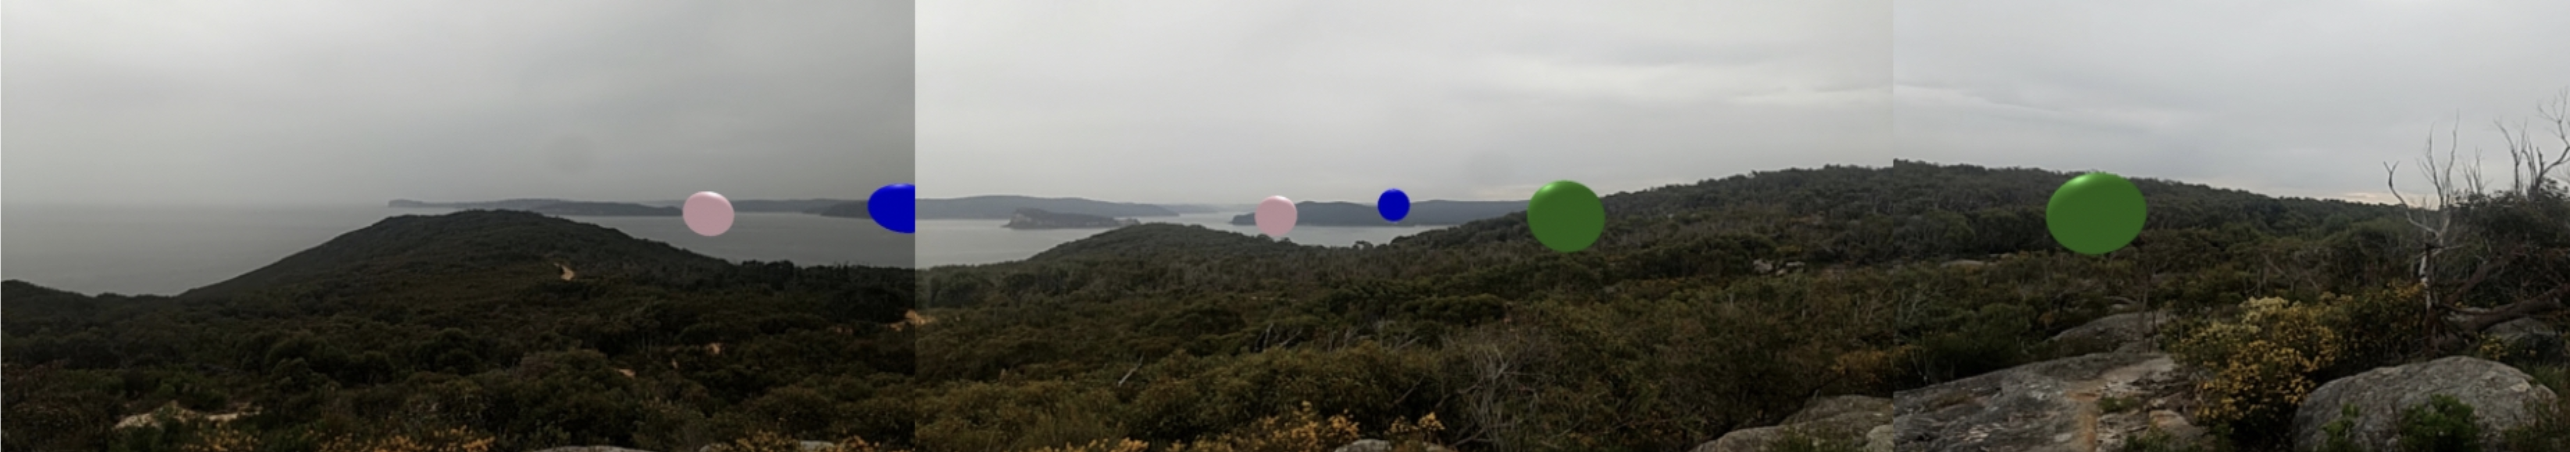
\includegraphics[width=3.31in]{paedomorphosis-bubble-sort.png}
    % \caption{Paedomorphosis: The simple geometries of the \emph{Algorithm} pieces were derived from sketches for an earlier piece involving placement of objects using GPS. \copyright Respect Copyright.}
    % \end{figure}

    % Paedomorphosis - The simple geometries of the Algorithms pieces came from the primitives I was using to position another piece of AR art.

\section{Conclusion}

    To think of art as a technology is to think across the fold that separates art from technology, towards a different way of partitioning of the sensible. The idea of art as a technology begins a process of smoothing out the fold. It challenges us to wonder what it would be like for the fold to not exist, potentially changing the way we think about both artmaking and our relationship with technology.
    
    We are invited to return to an idea of crafting, governed by ethics and informed by an appreciation of the complex, interconnected nature of reality and the rich, living agency of our various things. Perhaps, by thinking of art as a technology, we will begin to learn how to live differently with our technology. To paraphrase Simondon, we may begin to think of ourselves as
    
    \begin{quote}
        [...] inventors of technical and living objects. We coordinate and organise their mutual relation at the level of machines, between machines. We render them compatible, we are agents and translators of information from machine to machine, intervening within the margin of indeterminacy harboured by the open machine's way of functioning, which is capable of receiving information. We construct the signification of the exchanges of information between machines. Our rapport with the technical object is a coupling between the living and the non-living. \citep[p.xvi]{SimondonOnThMdOfExstncOfTechnclObjcts1980}
    \end{quote}

\bibliographystyle{isea}
\bibliography{isea}

\section{Author Biography}

Anonymous 

\end{document}

% \begin{quote}
%     I believe this asymmetry creates a high degree of preinformational directionality — a highly charged, saturated and unstable disparity that “wants” transductively to be discharged. Relative entropy thus contains a core element of self-differencing — as a range of potential options and occasional actualizations, the universe seems unable to do anything \emph{other than to create information}.
% \end{quote}

% Art itself is constantly evolving, generating new styles and discourses that increase the range of possible interpretations and creative options.

% \begin{quote}
%     [...] Each new stylistic and discursive development [...] increases the range of options available for future stages of artistic change while decreasing the ability to predict still further changes due to the increase of available options. In information theory terms, then, each such expansion increases the range of signal unpredictability — and thus information content — still further, creating an autocatalytic aesthetico-information feedback loop. \citep[p.2]{HoelscherThPtcsOfPhsSpc2014}

% \end{quote}
% \begin{figure}[h]
% 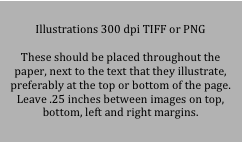
\includegraphics[width=3.31in]{figure.png}
% \caption{This is an example of figure caption. Note that all figures, and tables are to be referenced in the text. \copyright Respect Copyright.}
% \end{figure}

% \begin{figure*}
% 
\includegraphics[width=\textwidth]{two-column-figure.png}
% \caption{Example of a double-column figure with caption. \copyright Respect Copyright.}
% \end{figure*}

% Jason Hoelscher has argued that art, as a system of practice theory, is a complex adaptive system \citep[p.38]{HoelscherNtsOnAtctlytcAsthtcs2015}. It uses the concept of dynamic equilibrium to describe the balance between the drive for novelty and the gravitational pull of established patterns or “attractor basins” within this system \citep[pp.41-42]{HoelscherNtsOnAtctlytcAsthtcs2015}. This balance ensures that while art is perpetually evolving, it remains anchored within a broader discourse, allowing for the formation of information-entropic dissipative structures — artworks. These objects, rich in complexity and depth, invite continuous interpretation and re-interpretation, reflecting the co-evolutionary nature of artistic practice and theory as they adapt and respond to each other and to their changing contexts. 

% Hoelscher has also referred to art styles and to recurring motifs in art as attractors. For example:

% \begin{quote}
%     [...] the human figure constitutes an artistic attractor of great power and draw, being “an oscillatory limit cycle around which the system flows repeatedly” (Kauffman 1993, 176) \citep[pp.11-12]{HoelscherThPtcsOfPhsSpc2014}
% \end{quote}

% \begin{quote}
%     Art as we name and understand it in our societies — Art in the singular, with a capital A — was unknown to those who enjoyed themselves at the theatre, commissioned works from painters and sculptors, listened to religious concerts, or hired musicians for their feasts or ceremonies. This is not a merely lexical issue. Art did not exist as a common sphere of experience, not only because the practice of the arts was intended for different social purposes, but, above all, because these purposes were themselves part of a hierarchical division of human activities and of the human beings who engaged in them. \citep[p.25]{RanciereMdrnTms2022}
% \end{quote}

% The regime of representation is epitomised for Rancière by classical theatre, in which the two meanings of the word sense — sensing as in experiencing, and making sense as in to understand conceptually — are tightly coupled.

% \begin{quote}
%     The stage was thought of as a magnifying mirror where spectators could see the virtues and vices of their fellow human beings in fictional form. And that vision in turn was supposed to prompt specific changes in their minds: Molière’s Tartuffe supposedly taught spectators to recognize hypocrites; Voltaire’s Mahomet to fight for tolerance against fanaticism, and so on. Now, that ability to produce the dual effect of intellectual recognition and appropriate emotion was itself predicated on a regime of concordance inherent in representation.
% \end{quote}

% Art “as technics“, Sauvagnargues says, “concerns the way in which materials (matières) are captured and assembled into matter (matière) of expression.” \citep[p.75]{SauvagnarguesArtmchns2016}. However, art is not reducible to technics so that it does not require a specific kind of analysis \citep[p.74]{SauvagnarguesArtmchns2016}.


% Flack has referred to an earlier study in which she worked with a group of monkeys (pigtailed macaques) who used a silent, bared-teeth signal to communicate about their specific position in a power distribution, as if each individual monkey had a “power score”. The power score was a “course-grained representation of [...] an individual's fighting ability as collectively perceived by the group” \citep[p.5]{FlackCrsGrnng2017}. The power distribution was very stable\footnote{

%     During the study there was only one relationship reversal over the course of 5 months. \citep[p.1584]{FlackCntxtMdltsSgnlMnng2007}

% }. This silent bared-teeth signal was always used in interactions between only two monkeys and was only emitted by the monkey with a lower power score. Flack found that the signal occurred in two contexts:

% \begin{enumerate}
%     \item{
%         In response to aggression or threat of it
%     }
%     \item{
%         During pass-bys and approaches in the absence of any overt aggression or threatening behavior
%     }
% \end{enumerate}

% The first use case, when the signal was used during conflict, can be read in behaviourist terms as a simple stimulus response. In this case the signal functioned as an indicator of submission. Flack focused instead on the use of the signal during peaceful encounters and found that its use was always correlated with the position in the power distribution of each monkey. She has suggested that the signal, when used in this context “enabled communication about subordination, a pattern of behavior, rather than just submission in the present interaction” \citep[p.1584]{FlackCntxtMdltsSgnlMnng2007}.

% The pattern of power distribution within the social system of the monkeys was apparently functioning as a store of information about the relative capability of each monkey to win fights\footnote{

%     Presumably fighting ability correlates with some fitness parameters

% }. The signalling process was making the information available in an easy, low-energy (coarse-grained) form. There was no need for the monkeys to be constantly fighting in order to know where they are positioned, nor to remember the power distribution (to store it in their brain). A monkey only needed to maintain an awareness of their power score, which they gleaned from casual interactions and from watching the interactions of other monkeys\footnote{

%     The power score is not a number (of course) but an estimate of “the \emph{degree of consensus} in the group that they can win fights” \citep[p.5]{FlackCrsGrnng2017}.

% }. The stable power distribution, as it was continually reinforced through the network of interactions and signals, made possible otherwise costly conflict-management strategies, such as a kind of policing strategy in which the most powerful monkeys were unchallenged when they intervened to break up disputes \citep[p.5]{FlackCrsGrnng2017}.

% If Flack's distinction between \emph{coarse-graining in Nature} and \emph{coarse-graining by scientists} is valid, it would make the concept less useful. Addressing an imagined readership of scientists, Flack referred to ideas like temperature as “coarse-grainings that we as scientists impose on the system to find compact descriptions of system behaviour sufficient for good prediction.” In making a distinction between what scientists do and “how adaptive systems identify regularities and build effective theories to guide adaptive decision-making and behaviour”, Flack was apparently suggesting, or assuming, that communities of scientists working together to measure and observe phenomena are somehow not \emph{adaptive systems identifying regularities and building effective theories to guide adaptive decision-making and behavior}. Clearly they are, as Chang, Latour and Woolgar, and other philosophers and historians of science have shown\footnote{
    
%     See DeLanda's discussion of the way scientists produce theories, e.g. he quotes Alan Garfinkel (Forms of Explanation, pp. 53–8): “an object of explanation should be chosen which is stable under small perturbations of its conditions.” \citep[pp.161-162]{DeLandaIntnsvSci2013}

% }.

% Coarse-graining is a more useful concept if it is not divided into two different types, one for scientists and one for the rest of reality. Scientists are participants in a complex process that includes, depending on where one decides to draw the boundary, the full human and social context of particular scientists, science itself, various technologies, the phenomena under observation and even quantum entanglements. Flack's tendency to treat science as something separate from nature could perhaps be an example of course-graining. She has noted that components in a complex system can tune to a slow variable regardless of whether it actually does a good job of summarizing regularities. “Think”, she has advised us, ”of social institutions that are highly constraining and very hard to change” \citep[p.9]{FlackCrsGrnng2017}.

% In any case, those days are over.

% The American critic and philosopher of art Arthur Danto was one of the first to point out the absurdity of the idea that aesthetic experiences are synonymous with the experiences of beauty (and also that it is a kind of philosophical colonialism, since it requires a single subjective, culturally informed, experience to function as an objective definition \citep[p.124]{DantoEmbdMnngs2007}), and that a focus on beauty has had the effect of delegitimising the real diversity of aesthetic experiences artists routinely deploy \citep[p.59]{DantoThAbsOfBty2003}, which might be based in virtually any kind of observed quality, like cuteness \citep[p.28]{DantoThPhlsphclArt2005}, grunge, blandness \citep[p.126]{DantoEmbdMnngs2007}, disgustingness, eroticism, \citep[p.59]{DantoThAbsOfBty2003}, et cetera.

% A final example is Frank Stella's 1959 stripe paining \emph{The Marriage of Reason and Squalor II}. Which

% \begin{quote}
%     [...] appears to be as resolutely determinate and definite as a painting can be, a kind of no-nonsense record of the process of its own creation. The painting is simultaneously composed of, and comprises, two sets of twelve equally spaced and concentrically organized stripes, each of which is a flat uninflected brushstroke the width of the brush with which it was painted.
% \end{quote}

% Stella apparently described his goals for the painting in blunt terms as being to “keep the paint as good as it was in the can” \citep[p.38]{HoelscherArtAsInfrmtn2021}. He also said of it: “What you see is what you see” \citep[p.39]{HoelscherArtAsInfrmtn2021}. However, Hoelscher has suggested, the painting is not as simple as it appears.

% \begin{quote}
%     [...] By the time Stella painted his first stripe paintings in 1959, art's network of discursive entanglements had reached a state so charged with potential that it was able to produce artworks discursively coded as nondiscursive objects [...] each painting has been discursively coded as a simple and nondiscursive object, the simple nondiscursivity of which makes it discursively important according to a complex weave of artistic discourses built up over the course of a century.
% \end{quote}

% Hoelscher summed up the operation of Stella's painting in the same informational terms as the Morris sculpture and the Duchamp readymade.

% \begin{quote}
%     Enfolding multiple orders of operation that range from deadpan brushstrokes, to objecthood, to tautological statement, to large-scale discursive and cultural complexes of ideas, the Stella stripe painting + statement ensemble thus operates as a differential object, as a bundle of tightly entangled yet irresolvable differences that propagate still further difference.
% \end{quote}

% In the early 2000s, the mode of resonance between philosophical and scientific theories of complexity found conceptual form in the term \emph{complexity thinking}, which started to be used by scholars and practitioners working in fields like management theory, organisational change, health and education. At this time, Complex Adaptive Systems theory was filtering through into popular culture with memes like “chaos theory” and the concept of \emph{emergence} capturing the collective imagination. The term \emph{complexity thinking} expresses a sense of complexity as an intrinsic quality shared by diverse phenomena, and a sense of things being connected in unpredictable ways. The term acknowledges, according to Paul Cilliers and Kurt Richardson, the “...epistemological consequences of assuming the ubiquity of complexity” \citep{CilliersRichardsonCmplxtyScnc2001}. Complexity thinking describes an awareness that we can never fully know the dynamic interconnected processes at play within and between all phenomena. While it limits what we can reasonably claim to know, it also changes how we think about the world in ways that create new possibilities for knowing. 

% \begin{quote}
%     Having a basis in mechanism is a critical property of a coarse-grained description — it is “true” to the system. It is a simplification of the microscopic details. In principle, a coarse-grained description does not introduce any outside information to the subset of microscopic interactions over which it is performed [...] \citep[p.4]{FlackCrsGrnng2017}
% \end{quote}

% This paper examines how art might function, technically, by capturing our evolutionary capacity for aesthetic experience and deploying it to create meaning. The aim is to develop the idea of art as a technology so that it is available as a heuristic, a kind of effective theory\footnote{
%     An effective theory is one that is “able to organize phenomena under an efficient set of principles” and is also “not impossibly complex” \citep[p.1]{WellsEffctvThrs2012}. A good effective theory functions as a heuristic — a rule of thumb that can serve as a guide for action. The critical requirement is \emph{observational consistency} (an effective theory need not be even be true, as long as it works) \citep[p.71]{WellsEffctvThrs2012}.
% } that might open a space of possibility for us to have a different relationship with our technology.


Purpose is synonymous with Aristotle's concept of \emph{final cause}, and functions as an \emph{enabling constraint} \citep{JuarreroCsltyAsCnstrnt1998}, giving art objects meaning. Meaning\postnote{

    DeLanda pointed out that the word \emph{meaning} is used in two different ways: to denote significance (as in “this life has a meaning”) and signification (as in “this word has a meaning”) \citep{DeLandaCsltyAndMnng2018}. Two forms of knowledge \citep[p.43]{DeLandaCsltyAndMnng2018} Meaning as signification is the most relevant in an art context, although both may apply.

}, information (in the Simondonian sense), and aesthetic experience are all \emph{affect}. One person's embodied meaning \citep[p.125]{DantoEmbdMnngs2007}, is another's reorientational expansion and entanglement of aesthetic experience \citep[p.78]{HoelscherArtAsInfrmtn2021}.

Kant's formulation that art is “...purposive without purpose...” \citep[p.57]{KantCrtqOfJdgmnt} is reformulated by complexity thinking, revealing art to be purposive with purposes that are `...indeterminate, expansive, many layered, and multidimensional...” \citep[p.25]{HoelscherThPtcsOfPhsSpc2014}. The purpose of an art object is always open, both to addition and to change. 


Assemblage Theory enables us to recognise art, by its flexible boundaries and heterogeneous components, as an extremely deterritorialised assemblage. Art is a social system. The aesthetic regime is connected with all other social systems but maintains its identity — its autonomy — through codification. It is never possible to formalise the codes because they are always mutating. Boundaries in the aesthetic regime — say, between objects that are art and things that are not art — are extremely flexible. “Art exists as a separate world since anything whatsoever can belong to it” \citep[p.X]{RancièreAisthesis2013}. The system ot art consists of all art objects that have been and can be made, galleries, materials, artists, et cetera, as well as the diverse array of concepts, stories, and judgments that ascribe meaning to it. Wildly different objects created using diverse techniques for different purposes may be treated by the system as artworks. 

While the knob of territorialisation in DeLanda's parametrised model of assemblages is turned way down for art, the knob of codification is turned way up. The aesthetic regime is a system of codes. Like the genetic codes that govern life, the codes that define what is and what isn't art at different times and in different contexts are not reducible to a set of rules. They are always in flux around concepts and beliefs which are themselves unstable. At any single moment, the system is characterised by a plurality of intersecting attitudes, agreements, disagreements and manifestos about art and aesthetic experience — including disagreement about whether art is about aesthetic experience. 

Like all deterritorialised assemblages the art system is always in danger of capture — for example, by economic forces or by individuals.

A style is an attractor state in the art assemblage. Art styles are technical subdomains, the results of bifurcations — symmetry breaking events within the system \citep[pp.165-170]{HalsallSystmsOfArt2008} \citep[pp.10-11,41-42]{HoelscherNtsOnAtctlytcAsthtcs2015}. A style is a virtual continuum, a set of potential forms that can be actualised in the production of art objects according to certain combinations of enabling constraints and purposes.

Art evolves through complex combinatorial evolutionary processes. New styles are formed through the recombination of existing styles, the introduction of new materials and techniques, and the development of new purposes. The evolutionary processes of art are similar to those of biological evolution, including mutation, selection, exaptation, mutualisms, paedomorphosis and epigenesis. 

Artists are active forces in the evolutionary processes of art, the creation and maintenance of the codes that define what art is and what it can do. Referring to the painter Barnett Newman's famous quip “Aesthetics is for me like ornithology must be for the birds” \citep[p.253]{MattickAsthtcsAndAntAsthtcsInThVslArts1993}, Paul Mattick noted that ”...artists, unlike birds in the wild, are engaged in a cultural and therefore historically evolving activity. For this reason aesthetics is actually quite unlike ornithology. The birds do not, for example, question the concepts evolved by theorists to describe their activities” \citep[p.258]{MattickAsthtcsAndAntAsthtcsInThVslArts1993}.

\section{Contemporary Technology-based Art}\label{sec:ContemporaryTechnologyBasedArt}

    If we consider that the world is full of potential information, that the disorder of the world is “...a highly charged and catalytic mode of entropy akin to information entropy — not inert, but saturated to bursting with potentials that are oriented toward actualization.” \citep[p.72]{HoelscherArtAsInfrmtn2021}, then Contemporary art is a way of actualising certain information, of making certain relations visible. These relations may be fictional, speculative, false or even impossible. Art can actualise new potential realities, new ways of being, new ways of seeing. Or it can make visible the hidden relations of the world as it is.

    Art that utilises emerging technologies is, unavoidably, Contemporary. The purposes of technology-based art includes making visible the hidden relations of technological systems, and calling into being new socio-technological realities.
